\section{Introduktion} \label{exointro}
Et af de spørgsmål, der nok altid har optaget menneskeheden er, om vi er alene, eller der er andre som os et sted. Engang var svaret ja - vi har mødt både neanderthalere og andre menneskearter gennem tiden. Men i alle områder, vi har undersøgt godt nok, kan vi ikke længere finde andre, der minder særligt meget om os selv mht. tænkemåde og teknologi. Et andet spørgsmål, der altid har optaget os er, hvordan vi og verden omkring os opstod. Er der andre steder som dette? Vi har kigget mod stjernerne og undret os over, hvad der findes langt borte.

Nu har vi endelig teknikken til at undersøge disse spørgsmål mere i dybden ved at lede efter exoplaneter, som er planeter uden for Solsystemet. Indtil videre har fokus ligget på at detektere så mange planeter som muligt og karakterisere dem, hvilket er nemmest for de store og tunge, men i fremtiden vil vi blive bedre til at analysere de jordlignende planeter. \\

%Astrointro om det observerbare univers, nukleosyntese og planetdannelse
\noindent
For at diskutere astrofysik, er det nyttigt at kende nogle begreber:\\

\noindent
\textbf{Luminositet} eller lysstyrke er den totale energi $E$ et objekt udsender i alle retninger per tid $t$.
\begin{align}
    L=\dif{t}{E}
\end{align}
\noindent
\textbf{Flux} beskriver hvor meget af noget man opfanger over et bestemt areal - sagt med andre ord, hvor meget der strømmer igennem et areal. Ofte siger man bare flux, når man egentlig mener energiflux - altså hvor meget af kildens energi vi opfanger. Fluxen $F$ måles i denne sammenhæng som energi $E$ per tid $t$ og areal $A$.
\begin{align}
    F=\frac{1}{A}\pdif{t}{E}
\end{align}
Det svarer til hvor meget af luminositeten, man opfanger over et bestemt areal, fx. på Jorden. Hvis man har et bestemt areal at måle med, og flytter det længere væk fra kilden, bliver det ramt af færre fotoner, så fluxen skal aftage. Fluxen følger
\begin{align}
    F=\frac{L}{4\pi D^2}, \label{afstandskv}
\end{align}
hvor $D$ er afstanden til objektet. Dette kaldes \emph{Afstandskvadratloven}, da fluxen falder med kvadratet på afstanden. Så objekter, der er langt væk, ser vi meget svagt. Afstandkvadratloven ser sådan ud, fordi man antager at stjerner udtråler isotropt, det vil sige lige meget i alle retninger, hvorfor den målte flux i en afstand $D$ fra kilden, er den fra kilden udsendt flux, over hvor stort et areal den har spredt sig over, hvilket er overfladen af en kugle.

\iffalse
    \textbf{Intensitet} er et mål for for meget lys der bliver udsendt i en bestemt retning. Det minder om flux, der bare også er divideret med hvor stor en vinkel af himlen man måler på. Vinklen $\d\Omega$ kaldes rumvinklen (solid angle på engelsk). 
    \begin{align}
        I=\frac{\partial^3E}{\partial t \partial A \partial\Omega}
    \end{align}
    Det interessante ved intensitet er, at det er uafhængigt af hvor langt man er fra kilden. Afstandskvadratloven siger at fluxen vil aftage, men til gengæld vil kilden også fylde mindre på himlen, og de effekter opvejer hinanden, så intensiteten bliver konstant.
\fi
\subsection{Dopplerforskydning}
Du kender nok til, at når en ambulance kører forbi, så lyder sirenens tone højere, når den nærmer sig, og dybere når den kører væk. Det skyldes et fænomen kaldet \emph{Dopplerforskydning}. %Find gerne lydklip til undervisningen
Det skyldes at lydbølgerne, eller mere præcist bølgens bølgelængde, skubbes sammen eller strækkes ud, afhængigt af hvilken hastighed de udsendes med i forhold til lytteren. Hvis en ambulance kører mod dig, og du står stille, vil du høre bølgerne sammenpresset. Men hvis du selv kører med samme hastighed foran ambulancen, så vil du høre dem på samme måde, som de bliver udsendt - altså på samme måde, som hvis både du og ambulancen står stille, da det er den relative hastighed, som er afgørende.
\begin{figure}[h!]
	\centering
	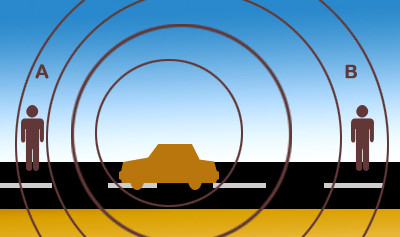
\includegraphics[width=0.5\textwidth]{Astrofysik/billeder/doppler.jpg}
	\caption{Dopplerforskydning af lyden fra en bil, der kører mod venstre. Person A vil høre en højere tone end person B, og personen i bilen vil høre noget et sted derimellem. Ringene viser et fast punkt på lydbølgerne.} % Kan man ikke ligeså godt skrive at ringene viser bølgetoppe, da det vel er dem man tegner pr. konvention?
	\label{doppler}
\end{figure}

Det samme sker for lys. Hvis en ambulance kører væk, vil både tonen blive dybere og lyset fra den en smule rødere, fordi bølgelængden bliver længere. Da rød svarer til lange bølgelængder og blå til korte (indenfor det synlige spektrum), så refererer rødforskydning til noget, som bevæger sig væk fra os og vice versa. 

Bemærk dog, at selvom fotoner og lydbølger har højere energi ved korte bølgelængder, så mister de ikke energi ved Dopplerforskydning - der er bare sket et skift i perspektivet, man ser bølgerne fra. Fra bølgens eget synspunkt (hvis man følger den) har den samme bølgelængde og energi hele tiden. På figur \ref{doppler} ses hvordan bølgerne "presses sammen" foran en kilde der bevæger sig, når man ser det fra et andet perspektiv.



\subsection{Spektre} \label{sec:spektrer}
Et spektrum viser intensiteten af lys ved forskellige bølgelængder eller frekvenser, fx som på figur \ref{spektrum}. Om bølger gælder det, at $v = f\lambda$, hvor $v$ er bølgens fart, $f$ er bølgens frekvens\footnote{Et andet almindeligt brugt symbol er det græske bogstav $\nu$, men her benyttes $f$, da det ikke minder så meget om det latinske bogstav $v$, der bruges om fart.} og $\lambda$ er bølgens bølgelængde. Lys bevæger sig med lysets fart, der afhænger af det medie lyset udbredes i, men det vigtige er, at den er kendt, hvorfor man simpelt kan regne $f$ ud fra $\lambda$ og omvendt. Pointen med dette er, at den eneste forskel på om et spektrum viser bølgelængde eller frekvens, er hvordan tallene skal fortolkes (fx vil spektret være spejlvendt, da de er omvendt proportionale).\footnote{For at gøre forvirringen total anvendes $\tilde{\nu} = \frac{1}{\lambda}$ også på nogle områder. Alt dette er traditioner og konventioner, der varierer fra område til område.} \\
\begin{figure}[h!]
	\centering
	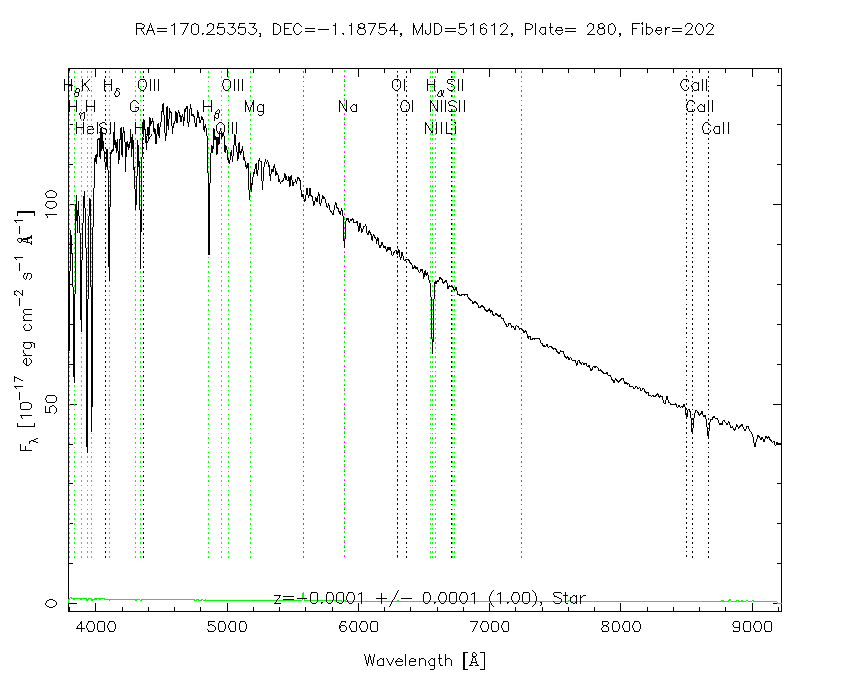
\includegraphics[width=0.7\textwidth]{Astrofysik/billeder/spektrum.png}
	\caption{Et typisk stjernespektrum. $y$-aksen skal forstås som intensitet, mens der
		på $x$-aksen er bølgelængde i Ångstrøm (\si{\angstrom}) (\SI{1}{\angstrom} = \SI{1e-10}{\metre}). Dykkene i intensitet
		er angivet med en overgang tilhørende et grundstof, som er identificeret i stjernens
		atmosfære.}
	\label{spektrum}
\end{figure}

I kapitlet Kvantemekanik blev tanken om kvantiserede energiniveauer introduceret, og denne teori videreføres i kapitlet Atom- og Molekylefysik til atomer. Eksempelvis er et hydrogenatom i et laboratorium på Jorden og et hydrogenatom i en stjerne langt væk i sidste ende samme grundstof, hvilket betyder, at de opfører sig ens, hvis de er udsat for samme betingelser. Det betyder, at man kan bruge sin viden om grundstofferne her på Jorden til at få viden om f.eks. stjerner i universet. \\
Lidt oversimplificeret kan det siges, at stjerner er så varme og tætte i kernen, at atomkerner har energi nok til at kunne overkomme deres indbyrdes elektriske frastødning.\footnote{Dette ville ikke være muligt, hvis det ikke var for kvantetunnelering. Kvantetunnelering er kort sagt, at partikler kan passere gennem en energibarriere for at komme hen til et område med lav potentiel energi. Dette svarer til at en bold kan komme forbi en meget stor bakke, som den egentlig ikke har nok energi til, for at komme hen på den anden side af bakken, hvor der er en dyb dal bolden gerne vil ned i. Dette kan jo ikke lade sig gøre for en bold, men det er essentielt set det der sker inde i stjerner hele tiden.} Når atomkernerne kolliderer, fusionerer de til en tungere kerne, hvilket frigiver energi. Dette kan lade sig gøre, fordi den specielle relativitetsteori siger, at masse og energi i virkeligheden er to sider af samme sag; $E=mc^2$. Denne energi kan danne lys, som passerer ud gennem stjernen, men det sker ikke uhindret. Der er langt fra stjernens centrum til dens overflade, og lys og atomer påvirker hinanden. Bliver et atom ramt af en foton med lige præcis nok energi til at excitere en elektron fra en tilstand til en anden, vil denne elektron skifte energiniveau. På et senere tidspunkt henfalder elektronen til en lavere energitilstand under udsendelse af den overskydende energi i form af en foton. Denne fotons energi er netop karakteristisk for overgangen mellem de to omtalte energiniveauer. I en stjerne er der mange atomer udenfor kernen, så når fotonerne skal igennem det, vil rigtig mange af de mulige excitationer ske. Så når lyset passerer igennem vil de bølgelængder der lige passer med energiforskellene absorberes, og derfor kan vi se de mangler, når vi kigger på stjernen. Ved at sammenligne med kendte energiforskelle fra forskellige grundstoffer og kemiske forbindelser i laboratoriet, kan vi bestemme hvilke stoffer, der har påvirket et spektrum, og hvor meget af hver.  \\

En fotons energi kan af ligning \eqref{kvant:fotonEnergi} udtrykkes som $E=hc/\lambda$, hvor $\lambda$ er fotonens bølgelængde, $h$ er Plancks konstant, og $c$ er lysets fart. Fordi energiforskellene mellem elektronbaner i et atom er helt specifikke, er de tilhørende bølgelængder det også. Da vi kender grundstofferne godt, ved vi hvilke energiniveauforskelle, der er karakteristiske for hvert atom, så vi også kan finde dem i spektret fra en stjerne. Når vi kan genkende energiforskellene fra et bestemt grundstof, kan vi dermed finde ud af hvad stjernens overflade består af, se figur \ref{spektrum}. Kigger man grundigt på denne figur ser man, at hver absorptionslinje, hvilket man kalder dykkene, har en udbredelse - de har ikke kun én bestemt bølgelængde. Dette skyldes en kombination af mange ting, hvoraf to af dem er Dopplerforskydningen og Heisenbergs usikkerhedsrelation\footnote{Den mest kendte af disse er relationen mellem sted og impuls, men der eksisterer en tilsvarende tid og energi.}
\begin{align}
    \sigma_E^2\sigma_t^2 \geq \frac{\hbar}{2}
\end{align}
Pga. usikkerhedsrelationen har energien en usikkerhed, så den ikke nødvendigvis er, præcis hvad vi ellers forventer. Derudover står atomer ikke stille i stjernen, men bevæger sig i alle mulige retninger, med vidt forskellige hastigheder og energier.\footnote{Partikler i en gas følger approksimativt Maxwell-Boltzmannfordelingen, hvilket den interesserede læser kan finde andet materiale om.} Effekten af dette er, at atomerne er i bevægelse, når de udsender fotonen, der senere observeres på Jorden, og Dopplereffekten er netop en forskydning af bølgelængderne, som følge af at kilden bevæger sig. Det at atomerne bevæger sig i alle mulige retninger, gør at Dopplerforskydningen trækker i alle mulige retninger, hvilket resulterer i en udbredning af linjen frem for et skift i dens placering. Jo varmere en gas er, desto hurtigere bevæger gassens atomer sig. Det vil sige at absorptionslinjerne fra en varm stjerne er bredere end dem fra en kold stjerne. Yderligere har stjernens temperatur også indflydelse på dens grundstofsammensætning, da nogle stjerner kan være så varme, at bestemte grundstoffer ikke er stabile. I forhold til exoplaneter er stjernens sammensætning blandt andet interessant, fordi den påvirker sandsynligheden for forskellige typer af planeter.